%
% Modelo LaTeX baseado no modelo A5L

% Nota: usar /newpage com 1 coluna
%       usar /clearpage com 2 colunas
%       o /newpage com duas colunas escreve na próxima coluna
\documentclass[a5paper,onecolumn, 11pt]{article}
\usepackage[landscape]{geometry}
\usepackage{indentfirst}
%Sample text
%\usepackage{lipsum}

%escrever acentos e coisas do género sem que o latex se desoriente
\usepackage[utf8]{inputenc}

%hifenização e titulos em portuguêsoa
\usepackage[portuguese]{babel}

%para ter a informação de quantas páginas tem o documento
\usepackage{lastpage}

%importar cores predefinidas
\usepackage[usenames,dvipsnames]{xcolor}
\definecolor{DarkGray}{gray}{0.40}

%usar multirow e multicolumn
\usepackage{multirow}

%hiperligações nas referências
\usepackage{hyperref}
\hypersetup{
    colorlinks,
    citecolor=blue,
    filecolor=blue,
    linkcolor=blue,
    urlcolor=blue
}
\hypersetup{linktocpage}

%para ter imagens, depois define a directoria de imagens
%\usepackage{graphicx}
\usepackage[pdftex]{graphicx}
\graphicspath{{imagens/}}

%escrever texto à volta de imagens
\usepackage{wrapfig}

%poder ter texto sublinhado que passa para a linha seguinte automaticamente
%usar com \uline{my underline text}
\usepackage[normalem]{ulem}

%definir o cabeçalho e rodapé
\usepackage{fancyhdr}
\pagestyle{fancy}
\fancyhead[L]{
    \small{
        \textcolor{DarkGray}{
            \textbf{Projecto Computação Gráfica}
        }
    }
}
\fancyhead[R]{
    \small{
        \textcolor{DarkGray}{
            \textbf{Pág. \thepage\ /\pageref{LastPage}}
        }
    }
}
\fancyfoot[C]{}

\begin{document}

\onecolumn
\thispagestyle{empty}
\begin{tabular}{ll}
    \multirow{7}{*}{ 
\includegraphics[height=90pt]{logo.jpeg} }
    &\\
    & \textcolor{DarkGray}{\Large{\textbf{Escola de Engenharia}}} \\
    &\\
    & \large{Departamento de Informática}\\
    &\\
    &\\
    & \large{Licenciatura em Engenharia Informática}\\
\end{tabular}
\begin{center}
    \Large{\textbf{Projecto de Computação Gráfica}}\\
    \vspace{20pt}
    \Large{\textbf{``Bar''}}\\
    \vspace{15pt}
    \begin{tabular}{r@{, }l}
        Bruno Ferreira&A61055\\
        Serafim Pinto&A61056\
    \end{tabular}
    
    \vspace{5pt}
    \emph{Grupo 19}\\\vspace{15pt}
    \large{\textbf{Braga, Maio de 2013}}
\end{center}

\newpage
\onecolumn
\tableofcontents
\newpage
\listoffigures

\newpage
\section{Resumo}
Neste relatório apresentamos todos os passos e decisões tomadas na construção do trabalho prático de Computação Gráfica.

Este projecto consiste na representação de um Bar, enquanto contrução geométrica. O Bar poderá conter elementos como mesas, cadeiras, copos, entre outros.

Numa primeira parte deste relatório fazemos uma breve introdução ao projecto, seguindo-se a análise do seu desenvolvimento ao longo das várias fases. Depois apresentamos uma descrição detalhada das técnicas usadas e, por fim, temos a conclusão.


\clearpage
\section{Introdução}
No desenvolvimento do presente projecto de Computação Gráfica pretendemos, para além de aplicar os conhecimentos leccionados na Unidade Curricular, desenvolver sensibilidade para a criação de aplicações de elevada complexidade gráfica. Propomos-nos portanto a criar um espaço com elementos comummente observados num Bar.

Este trabalho está dividido em quatro fases distintas. Na primeira fase apenas são feitas as primitivas: plano, cubo, cilindro, esfera. Numa segunda fase, devem ser apresentados alguns itens que deverão estar no espaço final, tais como: mesas, cadeiras, copos e candeeiros. A terceira fase consiste na preparação das primitivas das fases anteriores para a inclusão de texturas e iluminação. Nessa fase, devemos também optimizar o projecto utilizando \textit{Vertex Buffer Objects}. Na quarta e última fase deve ser montado o Bar propriamente dito, fazendo uso de tudo o que foi criado até ao momento. Além disto, a visualização do modelo deve ser feita recorrendo a uma câmara de movimento livre, com o uso do teclado e rato. Posto este problema, que está descrito no enunciado do trabalho, deveremos implementar e tornar possível a criação deste cenário seguindo os requisitos que serão apresentados no capítulo seguinte.

O projecto será desenvolvido em C++ no software Visual Studio 2012. Utilizaremos também a biblioteca gráfica do OpenGL, os utilitários GL (GLU), o GL Extension Wrangler (GLEW) e a extensão DevIL.

Para criação de texturas utilizaremos o software Genetica Viewer 3.5.


\clearpage
\newpage
\section{Descrição do Trabalho e Análise de Resultados}
Neste capítulo vamos descrever o desenvolvimento de cada um dos requisitos a ser apresentados. Descreveremos também os principais passos da sua implementação e estruturação e faremos uma breve análise dos resultados obtidos com estas mesmas implementações.


\newpage
\onecolumn
\subsection{Requisitos}
Durante esta secção apresentamos em detalhe os requisitos propostos em cada fase para o desenvolvimento do nosso projecto.
\subsubsection{Primeira Fase}
\begin{itemize}
    \item{Construir uma biblioteca de primitivas: plano, cubo, cilindro e esfera;}
    \item{Cada primitiva deve ser feita numa função que desenhe a primitiva centrada na origem;}
    \item{A função para cada primitiva deve ter um conjunto de parâmetros que permita desenhar de acordo com a dimensão e resolução pretendidas;}
    \item{Construção de uma aplicação OpenGL que permita a visualização de cada primitiva separadamente.}
\end{itemize}
\newpage
\subsubsection{Segunda Fase}
\begin{itemize}
    \item{Apresentar rotinas que desenhem os seguintes objectos: mesas, cadeiras, copos e candeeiros;}
    \item{Desenhar o espaço limite do bar, ou seja, paredes chão e tecto;}
    \item{À exceção do copo, todos os outros objectos devem ser desenhados à custa da biblioteca de primitivas da primeira fase, e de transformações geométricas. O copo deve ter uma rotina própria para a sua construção;}
\end{itemize}
\subsubsection{Terceira Fase}
\begin{itemize}
    \item{Definição das coordenadas de textura e definição das normais nas primitivas;}
    \item{Utilização de VBOs;}
    \item{Construção de  uma aplicação que permita a visualização de cada composição geométrica.} 
\end{itemize}
\newpage
\subsubsection{Quarta Fase}
\begin{itemize}
    \item{Aplicação com a apresentação da composição geométrica final, ou seja, um bar com mesas, candeeiros, cadeiras e copos (construídos apenas com recurso às primitivas e transformações geométricas desenvolvidas nas fases anteriores);}
    \item{Utilização de texturas e iluminação.}
    \item{Visualização da cena utilizando uma câmara de movimento livre, sem necessidade de detecção de colisões.}
\end{itemize}
\newpage
\subsection{Implementação}
Nesta seccção descrevemos de forma incremental o desenvolvimento do projecto ao longo das 4 fases.
\subsubsection{Primeira Fase}
A  primeira fase  pedia que fosse construída uma biblioteca com primitivas  geométricas, aqui explicamos  como nesta fase do projecto construímos cada uma delas. Estas primitivas foram numa classe à qual chamámos \textbf{Primitivas}. Para facilitar a visualização destas, elaborámos também uma \textit{main.cpp}, onde é possível através do teclado mover a câmara e visualizar o objecto de ângulos diferentes.

Criámos também o módulo \textbf{Utilities}, onde temos pequenas funções que nos facilitam na escrita do código tornado-o mais fácil de ler (p.e função que passa de graus para radianos). Além disto, temos um menu associado ao botão direito do rato onde o utilizador pode escolher qual a primitiva a visualizar, e visualizar o objecto de várias formas (figura colorida, apenas linhas ou apenas pontos).
\newpage
\begin{description}
	\item[Plano] \hfill \\
	A função que desenha o plano recebe como argumentos, o comprimento, a largura e ainda o número de camadas que o plano terá. Como queremos o nosso plano com um determinado número de camadas, dividimos as variáveis comprimento e largura pelas camadas pretendidas,  e guardamos o resultado em \textit{x2} e \textit{z2} respectivamente (sobre camadas, ver secção \ref{Camadas nas primitivas}).

	Como também queremos desenhar centrado na origem, dividimos o comprimento e a largura  por dois, e guardamos o resultado nas próprias variáveis. E é assim, com base nessas variáveis  que desenhamos os triângulos que compõem o nosso plano.
	A Figura 1 permite visualizar o nosso plano nesta fase:
	\begin{figure}[h!b!t!]
		\centering
		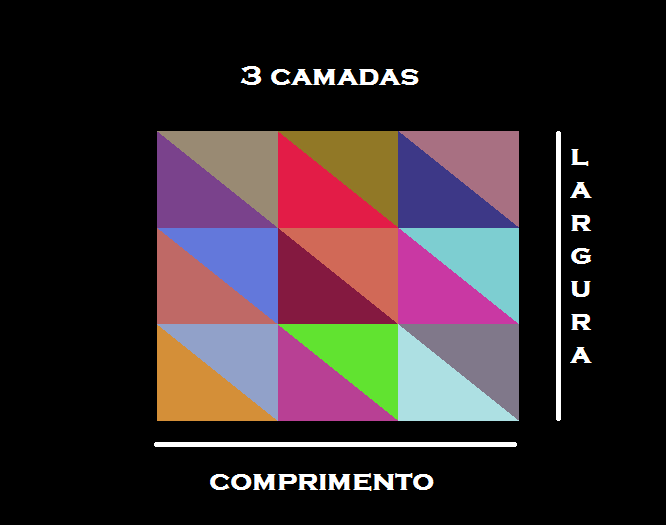
\includegraphics[scale=0.29]{plano.png}
		\caption{Plano com 5 de comprimento, 4 de largura e 3 camadas}
	\end{figure}
	\clearpage
	
	\item[Cubo] \hfill \\
	A função que desenha o cubo recebe como argumento o comprimento do lado e o número de camadas no eixo dos \textit{X} e dos \textit{Z}. Tal como no plano, para centrar o cubo na origem, a variável lado é dividida por dois. Para desenhar esta primitiva, como seria de esperar desenhamos seis faces, e cada uma delas desenhada da mesma maneira que é desenhado um plano.
	
	Optámos por criar um cubo e não um paralelipipedo, pois um paralelipipedo pode ser obtido escalando um cubo.
	
	Visto ser ineficiente, não recorremos à função que cria o plano para construir o cubo (ver secção \ref{evitar mudancas de estado})
	
	\item[Cilindro] \hfill \\
	Este primitiva foi desenhada de um método muito semelhante ao usado no execício da aula prática. A função recebe como argumentos o raio, a altura, o número de camadas verticais e o número de camadas horizontais. Existe uma varíavel \textit{delta} que resulta da operação
	\begin{verbatim}
	float delta = 2 * M_PI / fatias;
	\end{verbatim}
	Ficando guardada nesta variável o ângulo necessário para obter as coordenadas polares. Mais uma vez como a primitiva deve ser desenhada na origem, dividimos a altura por dois. O Cilindro é assim desenhado com recurso a coordenadas polares (ver secção \ref{CoordenadasPolaresEEsfericas}). Posteriormente o cálculo deste ângulo foi modificado para passar a ser calculado a cada iteração para evitar erros de vírgula flutuante (ver secção \ref{Erros de virgula flutuante}).

	\item[Esfera] \hfill \\
	A função que desenha esta primitiva recebe três argumentos: o raio da esfera, o número de camadas verticais e o número de camadas horizontais. É através de dois ângulos e funcões trignométricas que conseguimos desenhar a primitiva. Estas variáveis são:
	\begin{verbatim}
		float alpha = 2 * M_PI / fatias;
		float beta = M_PI / seccoes;
	\end{verbatim}
	Estamos agora a utilizar coordenadas esféricas (ver secção \ref{CoordenadasPolaresEEsfericas}). Existem três ciclos, um que desenha a parte de baixo, outro que desenha a parte de cima e por fim um que desenha as secções intermédias.
	Posteriormente o cálculo destes ângulos foi modificado para passar a ser calculado a cada iteração para evitar erros de vírgula flutuante (ver secção \ref{Erros de virgula flutuante}).
	\begin{figure}[h!b!t!]
		\centering
		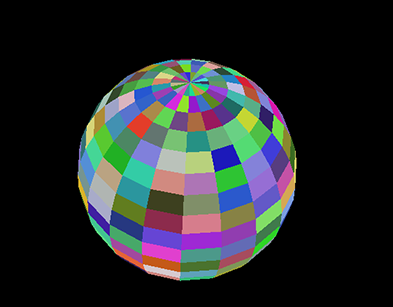
\includegraphics[scale=0.7]{esfera.png}
		\caption{Esfera com 2 de raio, 20 camdas horizontais e verticais}
	\end{figure}
\end{description}
\clearpage
\subsubsection{Segunda Fase}
Em relação à primeira etapa, reoganizámos o nosso trabalho com o objectivo de ter uma melhor organização e escalabilidade. Para isso foram criadas algumas novas classes.

Criámos uma classe \textbf{CG\_OBJ} que define um \textit{Vertex Buffer Object} (sem índices). De forma simplificada, um \textit{VBO} é buffer onde se guarda um conjunto de vértices correspondente a uma primitiva (ver secção \ref{VBO}).

Para compor vários \textit{VBO} de modo a formar um objecto complexo foi criada a classe \textbf{Figuras}. Esta classe \textit{static} apenas tem um \textit{array} de \textbf{CG\_OBJ} e métodos que compõem elementos desse array para formar figuras complexas. Estes métodos são utilizados pelo \textit{renderScene()} para desenhar objectos construidos por composição de primitivas.

Foram também criadas sub-classes da classe \textbf{CG\_OBJ} correspondentes às várias primitivas: \textbf{Plano}, \textbf{Cubo}, \textbf{Cilindro} e \textbf{Esfera}. De notar que a forma de desenhar as primitivas mudou e, como tal, a nova forma de desenhar primitivas difere consideravelmente da forma que constava na classe \textbf{Primitivas}. Além das quatro primitivas, foi adicionada a classe \textbf{SolidoRevolucao} que foi usada para desenhar copos (ver secção \ref{SolidosRevolucao}).

Também implementámos uma câmara FPS (ver secção \ref{camara fps}) e alterámos a interacção através do teclado com a aplicação (ver secção \ref{Gestao de input}). De forma a aumentar a escalabilidade do projecto, criámos duas novas classes para o controlo da câmara e teclado. São respectivamente a classe \textbf{Camera} e a classe \textbf{Input}. Ao longo das fases seguintes, ambas as classes \textbf{Camera} e \textbf{Input} foram sofrendo alterações conforme foi necessário.
\newpage
\begin{description}
	\item[Espaço limite do Bar] \hfill \\
	Para simular o espaço do Bar, fizemos com que toda a cena fosse desenhada dentro de um cubo com as seis paredes visíveis.
\begin{figure}[h!b!t!]
	\centering
	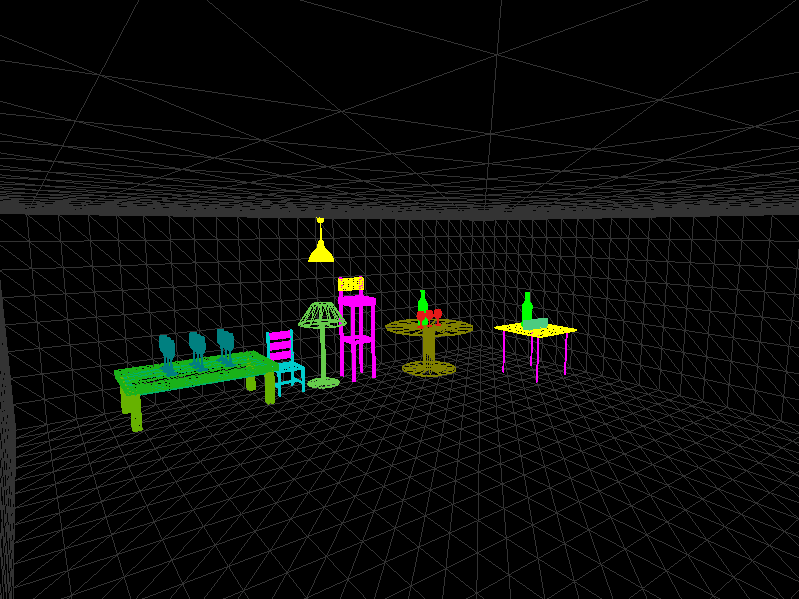
\includegraphics[scale=0.4]{paredes.png}
	\caption{As seis paredes visíveis em modo linha}
\end{figure}
\newpage
\item[Objectos] \hfill \\
Para além do espaço limite do bar, foi também pedido que fossem construídos alguns elementos que se podem encontrar num bar. Estes elementos são desenhados recorrendo aos métodos da classe \textbf{Figuras}.

Para esta fase desenhámos três \textbf{mesas}, sendo que uma delas tem a base e o tampo redondo, outra mesa \textbf{quadrada} e por fim uma mesa \textbf{rectângular} baixa.

A mesa \textbf{quadrada} é a mais simples das três, contendo quatro cilindros que constituem as pernas da mesa e um rectângulo para a superfície.

Temos uma mesa rectangular mais baixa que a quadrada. A mesa é formada por 9 cubos: 4 para as pernas, 4 para o reforço e 1 para a superfície da mesa.

Por fim temos a mesa \textbf{redonda}, que é composta por uma base de suporte inferior e pela superfície superior. A unir estes itens está um cilindro de raio inferior à base e ao tampo. Esta mesa é desenhada com recurso a Sólidos de Revolução (ver secção \ref{SolidosRevolucao}).

Outro elemento do Bar pedido eram as \textbf{cadeiras}, além de cadeiras optámos por também desenhar um \textbf{banco} alto. As pernas, assento e recosto da cadeira são cubos. O banco tem pernas cilíndricas e ambos o recosto e o assento são cubos.
\begin{figure}[h!b!t!]
    \centering
    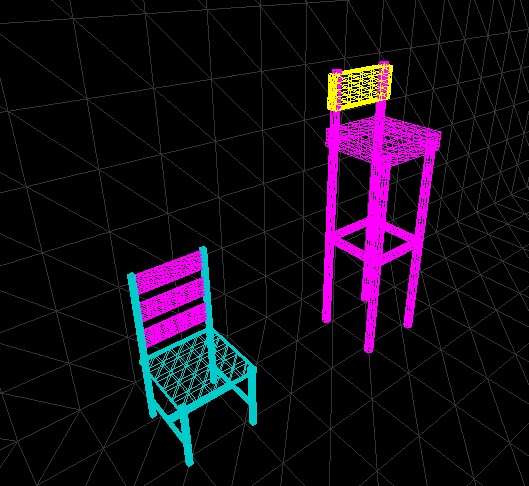
\includegraphics[scale=0.7]{cadeiras.png}
    \caption{Cadeira normal e banco de balcão}
\end{figure}

Apresentamos agora os \textbf{copos} que criámos usando Sólidos de Revolução (ver secção \ref{SolidosRevolucao} para detalhes sobre Sólidos de Revolução). Recorrendo à mesma técnica desenhámos também uma garrafa.
\begin{figure}[!htb]
    \centering
    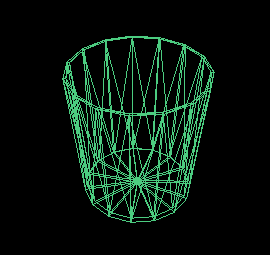
\includegraphics[scale=0.8]{copo.png}
    \caption{Copo simples}
\end{figure}
\begin{figure}[!htb]
    \centering
    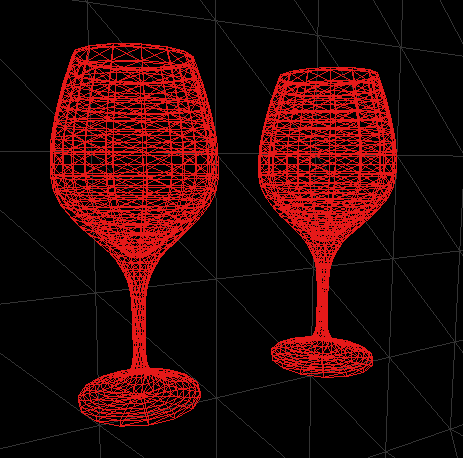
\includegraphics[scale=0.6]{vinho.png}
    \caption{Copo de vinho}
\end{figure}
\begin{figure}[!htb]
    \centering
    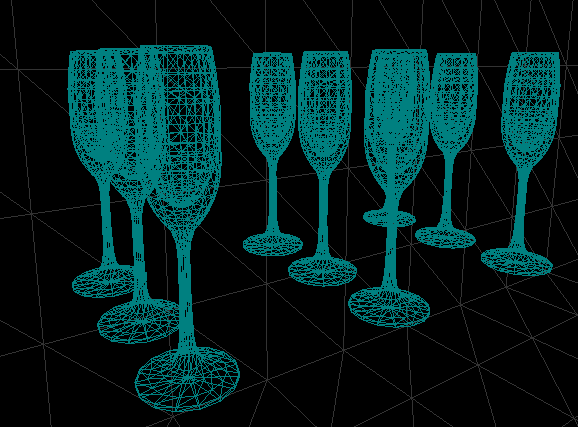
\includegraphics[scale=0.7]{champanhe.png}
    \caption{Copos de champanhe}
\end{figure}
\begin{figure}[!htb]
    \centering
    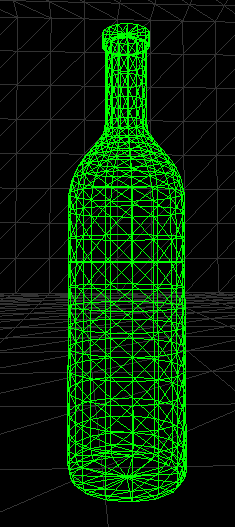
\includegraphics[scale=0.7]{garrafa.png}
    \caption{Garrafa}
\end{figure}

Finalmente o último item pedido eram candeeiros, aqui optámos por fazer dois estilos diferentes, um de tecto e outro de pé. Tanto o candeeiro de tecto e o \textit{abajour} do candeeiro de pé são Sólidos de Revolução. O candeeiro de pé também é formado por uma composição de vários cilindros.
\begin{figure}[!htb]
	\centering
	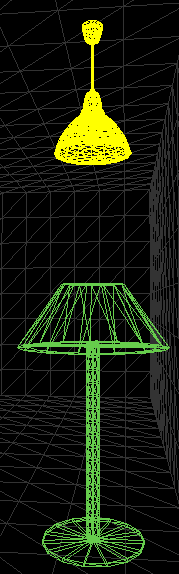
\includegraphics[scale=0.6]{candeeiros.png}
	\caption{Candeeiro de tecto e de pé}
\end{figure}
\end{description}
\clearpage
\subsubsection{Terceira Fase}
Tal como já tinha sido referido anteriormente e no enunciado, um dos objectivos para esta etapa do projecto seria a utilização de \textit{Vertex Buffer Objects} no desenho do Bar. Os \textit{VBO}s que implementámos não são óptimos, pois não utilizam indices. Nesta fase serão implementados \textit{VBO}s com indices (ver secção \ref{VBO}).

\begin{description}
	\item[\textit{VBO}s nas Primitivas] \hfill \\
	Já tinhamos os \textit{VBO}s implementados na segunda fase, portanto nesta fase apenas implementámos indices e adicionámos coordenadas de textura e normais aos vértices.
	
	Nesta fase a classe \textbf{Figuras} continua a ser responsável pela composição de \textbf{CG\_OBJ} em objectos complexos.
	
	\item[Iluminação e Texturas] \hfill \\
	Utilizando as coordenadas de textura e as normais aos vértices nos \textit{VBO}s implementámos texturas e iluminação no nosso Bar. Para não comprometer a escalabilidade do projecto, foram criadas duas novas classes: \textbf{Texturas} e \textbf{Light}. 

\end{description}
\newpage

\begin{figure}[!htb]
    \centering
    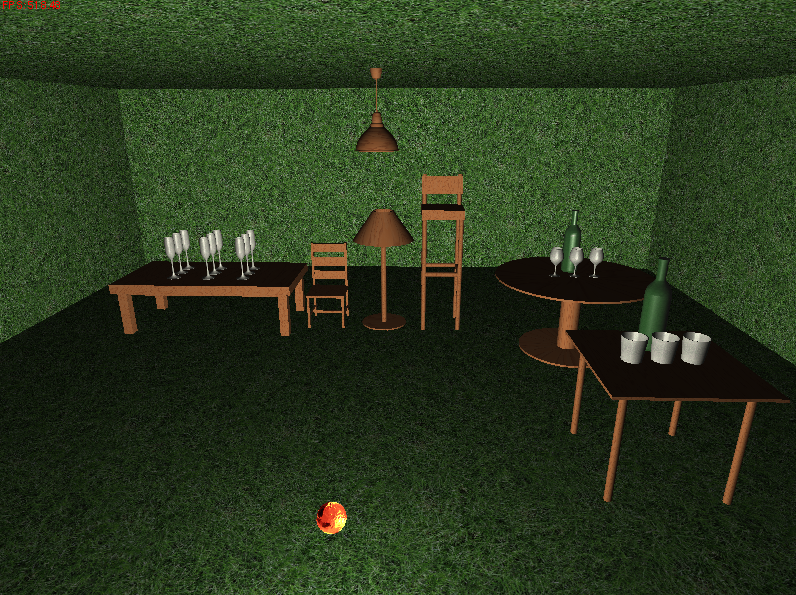
\includegraphics[scale=0.5]{fase3.png}
    \caption{Composição do Bar no fim da fase 3}
\end{figure}

\clearpage
\subsubsection{Quarta Fase}
Nesta fase deve ser apresentado o produto final deste projecto: o Bar. Para esta fase também nos é sugerido que exista iluminação, texturas e uma câmara de movimento livre.

\begin{description}
	\item[Visualização da cena utilizando uma câmara de movimento livre] \hfill \\
	A câmara estilo FPS está implementada desde a segunda fase sob a forma da classe \textbf{Camera}. Esta classe tem sofrido alterações de acordo com as necessidades. Nesta quarta fase a \textbf{Camera} também está encarregue de actualizar os planos do View Frustum (ver secção \ref{view frustum culling} sobre View Frustum Culling).
	
	\item[Utilização de texturas e iluminação] \hfill \\
	As texturas e a iluminação foram implementadas na fase anterior. Nesta fase apenas sofreram alterações para adicionar texturas ou facilitar o uso da classe.
	
	\item[Aplicação com a apresentação da composição geométrica final] \hfill \\
	Depois de compostas as várias primitivas criadas ao longo do projecto, obtemos o produto final: o Bar.
\end{description}

\newpage
\begin{figure}[!htb]
    \centering
    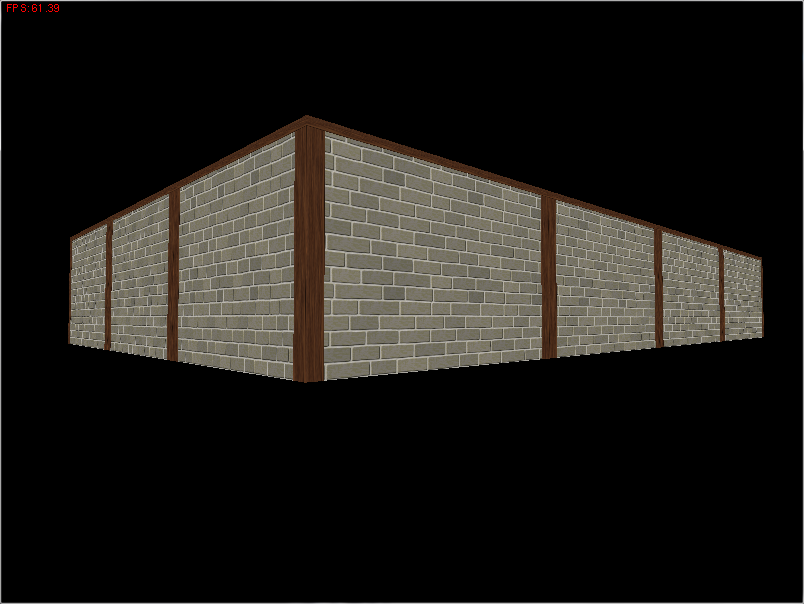
\includegraphics[scale=0.5]{bar9.png}
    \caption{Parede exterior}
\end{figure}
\begin{figure}[!htb]
    \centering
    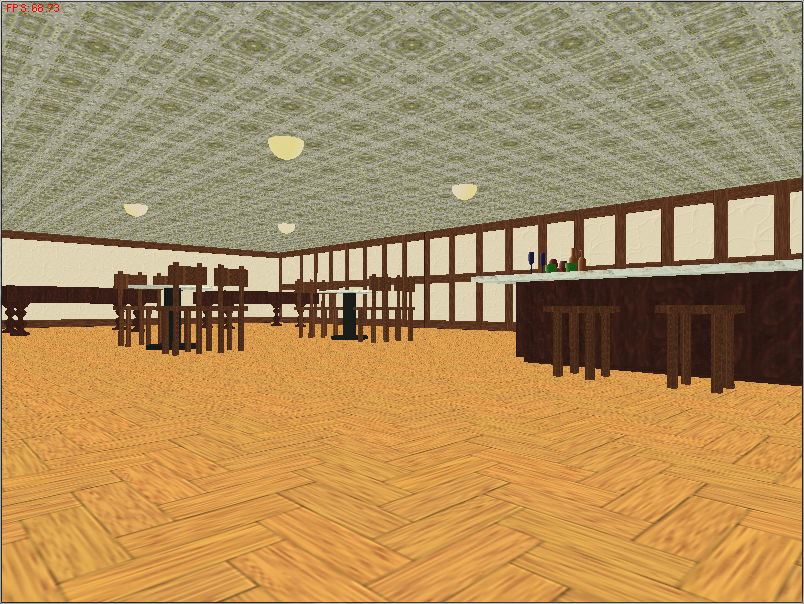
\includegraphics[scale=0.5]{bar1.png}
    \caption{Perspectiva geral sobre o bar}
\end{figure}
\begin{figure}[!htb]
    \centering
    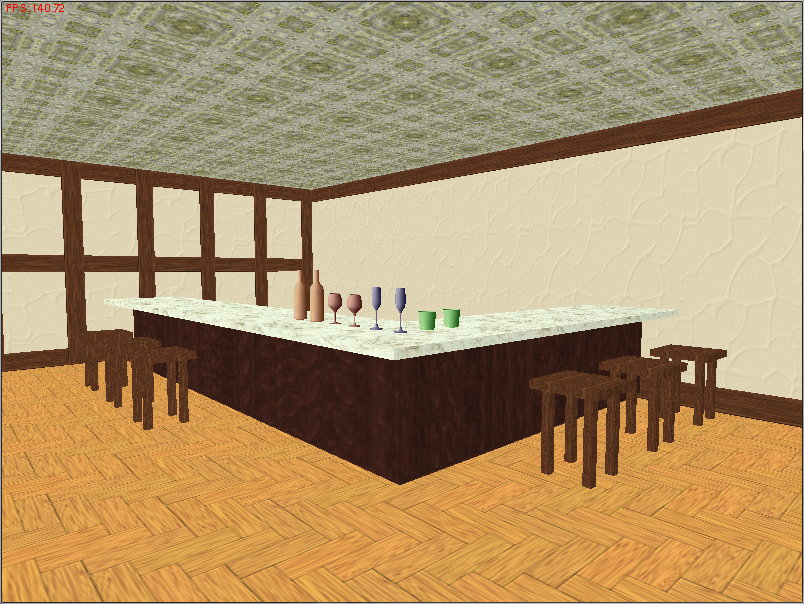
\includegraphics[scale=0.5]{bar2.png}
    \caption{Balcão, copos, garrafas e bancos}
\end{figure}
\begin{figure}[!htb]
    \centering
    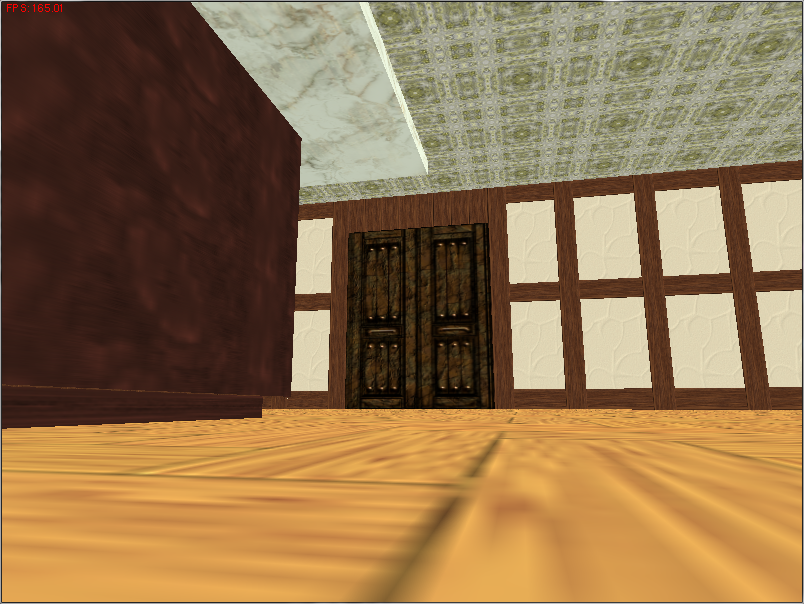
\includegraphics[scale=0.5]{bar10.png}
    \caption{Pormenores do balcão e porta}
\end{figure}
\begin{figure}[!htb]
    \centering
    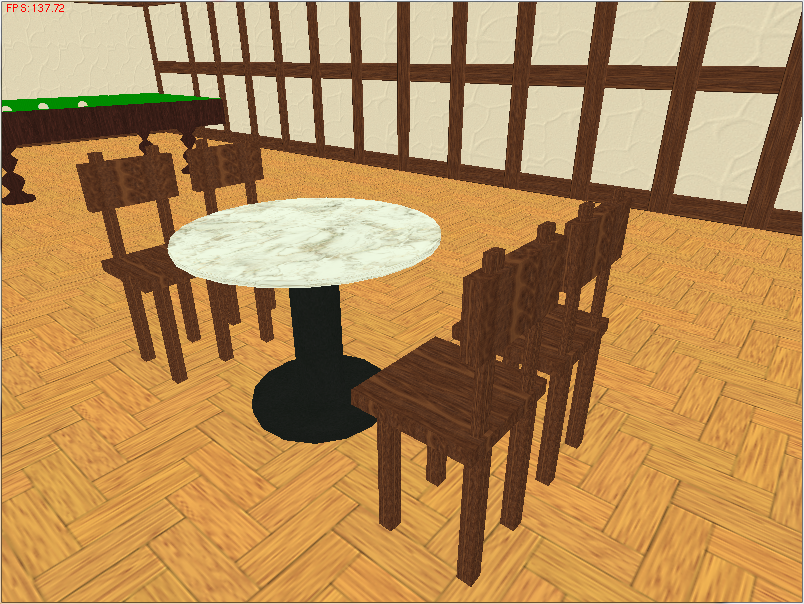
\includegraphics[scale=0.5]{bar3.png}
    \caption{Mesa e cadeiras}
\end{figure}
\begin{figure}[!htb]
    \centering
    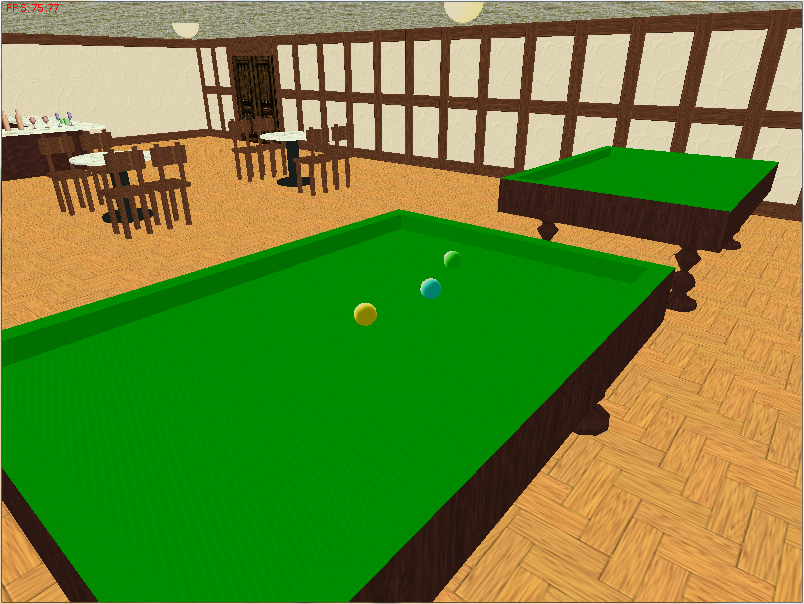
\includegraphics[scale=0.5]{bar4.png}
    \caption{Mesas de bilhar com bolas}
\end{figure}
\begin{figure}[!htb]
    \centering
    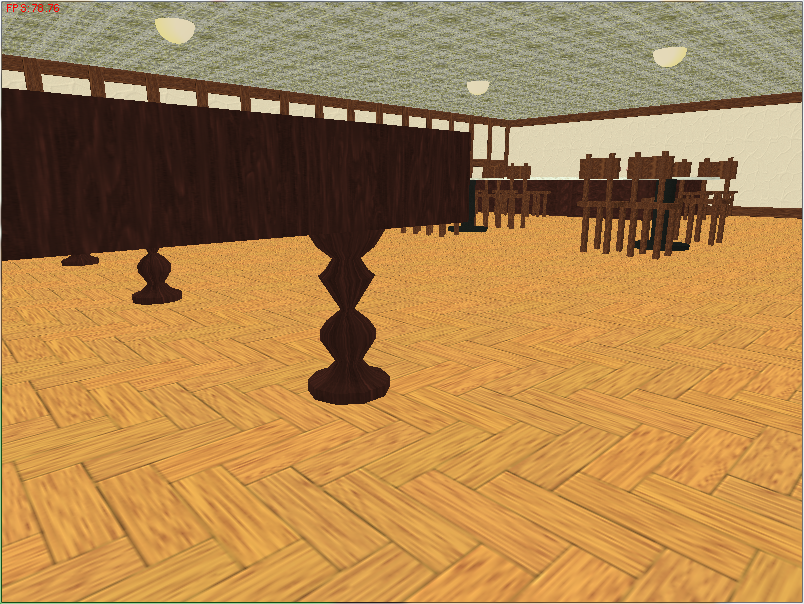
\includegraphics[scale=0.5]{bar5.png}
    \caption{Pormenor das pernas da mesa de bilhar}
\end{figure}
\begin{figure}[!htb]
    \centering
    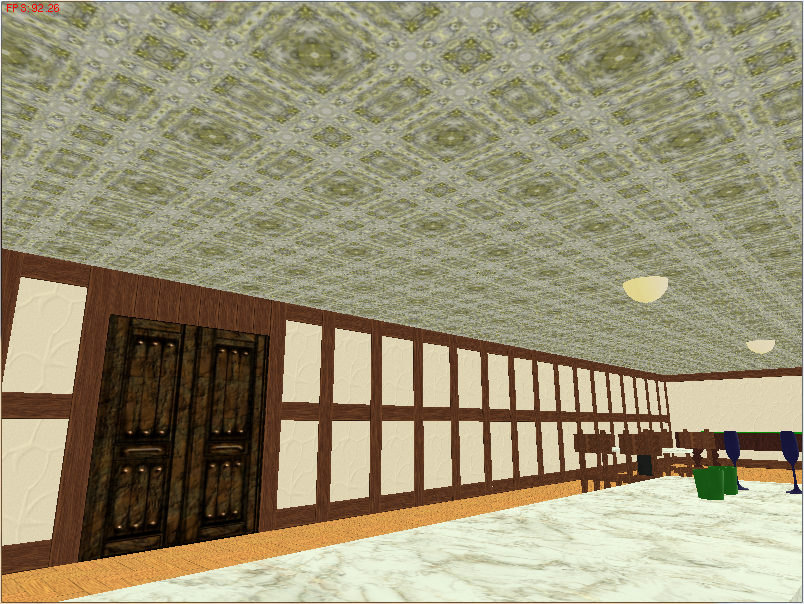
\includegraphics[scale=0.5]{bar6.png}
    \caption{Porta, decoração da parede, tecto e candeeiros }
\end{figure}
\begin{figure}[!htb]
    \centering
    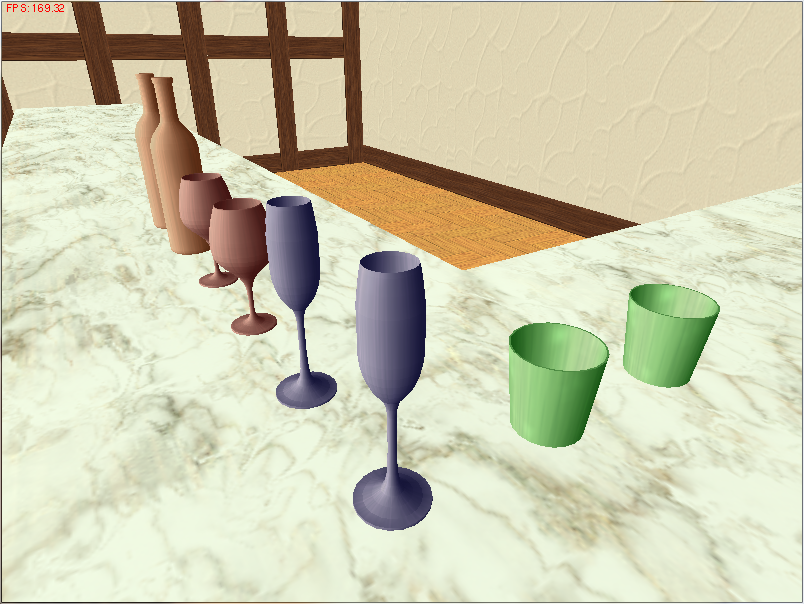
\includegraphics[scale=0.5]{bar7.png}
    \caption{Os copos e garrafas}
\end{figure}
\begin{figure}[!htb]
    \centering
    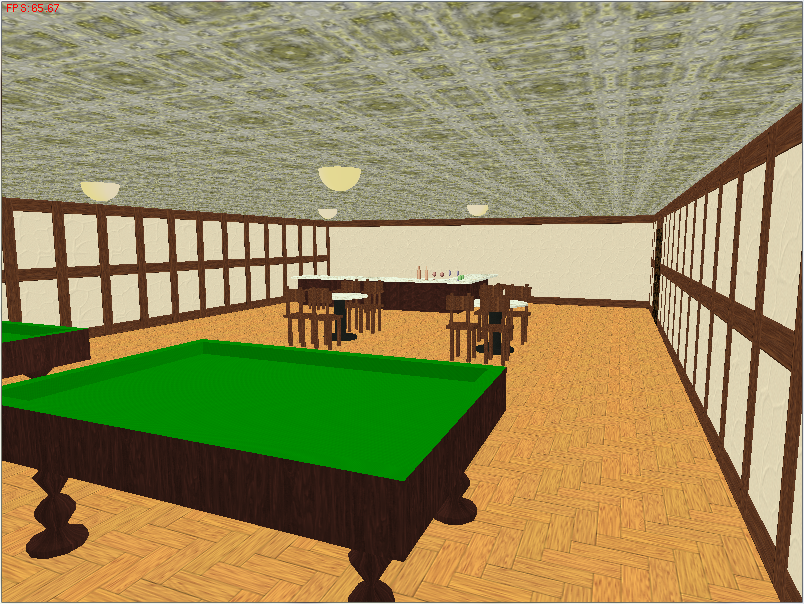
\includegraphics[scale=0.5]{bar8.png}
    \caption{Perspectiva da outra mesa de bilhar}
\end{figure}

\newpage
\clearpage
\section{Navegação e Controlos}
Apresentamos agora os controlos relativos à etapa final do projecto. Estes controlos são responsabilidade das classes \textbf{Camera} e \textbf{Input}.

\begin{description}
	\item[Teclas W,S,A e D] \hfill \\
	A câmara é movimentada utilizando as teclas  A,W,S e D para deslocar a câmara para a esquerda, para a frente, para trás e para a direita, respectivamente.
	
	\item[Movimento do rato] \hfill \\
	O movimento do rato permite "olhar em volta".
		
	\item[Tecla Z] \hfill \\
	A tecla Z permite alternar entre um modo de visualização em que apenas são desenhadas linhas e o modo de desenho natural.
		
	\item[Tecla X] \hfill \\
	A tecla X permite activar e desactivar o View Frustum Culling.
	
	\item[Barra de Espaços] \hfill \\
	A barra de espaços permite activar ou desactivar o modo de câmara FPS.
	
	\item[Tecla + e --] \hfill \\
	Aumentar e reduzir a velocidade de descocação da câmara.
\end{description}

\newpage
\section{Optimização e Técnicas usadas}
Apresentamos agora uma descrição pormenorizada sobre as técnicas usadas e optimizações.

\subsection{Evitar erros de vírgula flutuante} \label{Erros de virgula flutuante}
As variáveis \textit{float}, ou de vírgula flutuante, têm uma precisão limitada. Esta limitação provoca, por vezes, efeitos inesperados ao calcular certos valores. Esta precisão limitada é uma falha aparentemente insignificante, mas que pode causar problemas quando há um acumular de erros de precisão.

Tomemos por exemplo a expressão $ x = 1*(0.5 - 0.4 - 0.1) $. É para nós óbvio que $x=0$, mas quando representado em formato de vírgula flutuante em binário, obtemos um valor possivelmente inesperado: $x = (-2.78*10^{-17})$ ou, de forma mais extensa, $x = -0.0000000000000000278$. Isto acontece porque o valor $0.1$ (como muitos outros valores) não é representável em formato de vírgula flutuante. Dependendo da utilização futura do nosso $x$, poderiamos ter erros na ordem dos milhões com alguma facilidade.


Para evitar estes erros substituem-se somas sucessivas por multiplicações.

Esta técnica é usada em vários ciclos da aplicação, principalmente quando existem ciclos \textit{for} cujo incremento é um ângulo. Nestes casos tenta-se obter o valor desejado à custa de uma multiplicação em vez de incrementos sucessivos.

\newpage
\subsection{"Camadas" nas primitivas} \label{Camadas nas primitivas}
As camadas nas primitivas são uma forma de assegurar que um triângulo nunca fica muito "esticado". Quando um triângulo fica demasiado esticado o \textit{openGL} tem dificuldade em calcular a iluminação para alguns pontos do triângulo e isso provoca um efeito irrealista ao desenhar.

\subsection{Coordenadas Polares e Esféricas} \label{CoordenadasPolaresEEsfericas}
Na matemática, o sistema de coordenadas polares é um sistema de coordenadas bi-dimensional no qual qualquer ponto de uma circunferência é determinado a partir de um ângulo e um raio.

\begin{figure}[!htb]
    \centering
    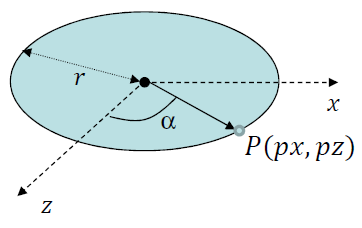
\includegraphics[scale=0.5]{coordPolares.png}
    \caption[Coordenadas Polares]{De acordo com a figura, temos que qualquer ponto \hbox{$P = (x,y)$} na circunferência pode ser represetado sob a forma \hbox{$P = ( r * sen(\alpha), r * cos(\alpha)$}}
\end{figure}

\clearpage
De forma análoga, temos que um sistema de coordenadas esféricas é um sistema de coordenadas tri-dimensional no qual qualquer ponto da esfera é determinado a partir de dois ângulos e um raio.
\begin{figure}[!htb]
    \centering
    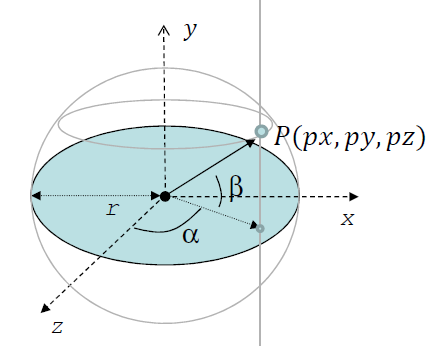
\includegraphics[scale=0.5]{coordEsfericas.png}
    \caption[Coordenadas Esféricas]{De acordo com a figura, temos que qualquer ponto \hbox{$P = (x,y,z)$} numa esfera de raio $r$ pode ser represetado sob a forma \hbox{$P = (r*cos(\beta)*sen(\alpha), r*sen(\beta), r*cos(\beta)*sen(\alpha))$} para \hbox{$-90 < \beta < 90$}}
\end{figure}

As coordenadas polares são utilizadas no cálculo dos vértices do cilindro e nos sólidos de revolução (ver secção \ref{SolidosRevolucao}). As coordenadas esféricas são utilizadas no cálculo dos vértices da esfera e no movimento da câmara.

\clearpage
\newpage
\subsection{Gestão de input} \label{Gestao de input}
O input é gerido na classe \textbf{Input}. Essa gestão consiste em ter um \textit{array} de $256$ booleanos (correspondentes aos 256 caracteres da tabela ASCII) que têm o valor \textit{true} caso a tecla correspondente esteja pressionada, ou \textit{false} caso contrário.

Desta forma, a cada frame, é chamado um método da classe \textbf{Input} que realiza acções conforme determinadas teclas estejam pressionadas. Esta abordagem, em conjunto com a directiva \textit{glutIgnoreKeyRepeat(1)}, permite (por exemplo) que o utilizador movimente a câmara simultaneamente em mais que uma direcção.

De notar que esta gestão depende do \textit{frame rate}, ou seja, quanto mais imagens por segundo forem produzidas, mais rápido é o movimento da câmara. Inicialmente, a implementação da classe input era baseada num temporizador que a cada 10 milisegundos realizava acções conforme as teclas pressionadas, desta forma o movimento da câmara era independente do \textit{frame rate}, mas em contrapartida processávamos as teclas pressionadas várias vezes por imagem.

\subsection{Câmara FPS} \label{camara fps}
A câmara FPS é uma implementação de coordenadas esféricas.

Imagine-se a câmara colocada no centro de uma esfera de raio $r=1$. Quando se move o rato, os ângulos $\alpha$ e $\beta$ são actualizados e, na próxima chamada à função \textit{gluLookAt}, o ponto \textit{center} para onde a câmara está apontada será calculado utilizando Coordenadas Esféricas, o raio $r=1$ e os ângulos $\alpha$ e $\beta$.

O movimento da câmara FPS também usa os mesmos ângulos $\alpha$ e $\beta$. Para mover a câmara (por exemplo) para a frente, o ponto $P$ da posição da câmara é deslocado na direcção do vector \textit{center} uma determinada quantidade de unidades.

\subsection{Sólidos de Revolução} \label{SolidosRevolucao}
Os sólidos de revolução são uma metodologia para desenhar uma vasta gama de figuras.

\begin{figure}[!htb]
    \centering
    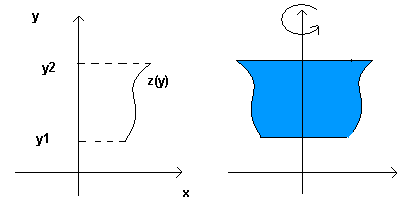
\includegraphics[scale=0.5]{solidoRev.png}
    \caption[Demonstração de Sólido de Revolução]{Para desenhar um sólido de revolução é necessário que a aplicação tenha conhecimento de uma lista de pontos sob a forma \hbox{$P=(x,y)$}. Depois de ter os pontos, a aplicação une-os, ordenadamente, e roda-os em torno do eixo dos $yy$.}
\end{figure}

O cálculo das normais dos sólidos de revolução produz normais de forma a suavizar a transição de um segmento do sólido de revolução para o próximo.

\clearpage
\subsection{Evitar mudanças de estado} \label{evitar mudancas de estado}
As placas gráficas processam os vértices em paralelo e de forma extremamente rápida, mas de cada vez que é necessário alterar o estado do \textit{openGL} (p.e para mudar a cor dos vértices a desenhar), é necessário esperar que todos os processadores da placa gráfica acabem de processar os vértices actuais, para depois efectivamente mudar o estado e fornecer mais vértices à placa. Este processo atrasa a operação de desenho dos vértices.

Esta é a razão pela qual (por exemplo) um cubo não deve ser construido a partir de rotações de planos.

\subsection{Vertex Buffer Objects} \label{VBO}
Os \textit{Vertex Buffer Objects}, ou \textit{VBO}s, são uma forma de optimizar um projecto de computação gráfica.

Os \textit{VBO}s são buffers na memória da placa gráfica onde é colocado um conjunto de vértices de forma a tornar o desenho desses vértices mais rápido. Os buffers são inicializados e são transferidos os vértices para o buffer apenas uma vez, na inicialização da aplicação. Quando houver necessidade de desenhar um objecto cujos vértices estejam guardados num \textit{VBO}, apenas é necessário que a placa gráfica os carregue a partir da sua memória reservada e os desenhe.

No modo de desenho imediato, os vértices são enviados para a placa gráfica uma vez por \textit{frame}, para depois serem desenhados. Com \textit{VBO}s os vértices são enviados para a placa apenas uma vez, reduzindo assim o custo de desenho dos vértices para um mínimo.

Os \textit{VBO}s "com indices" são outra optimização que se pode fazer que evita que a placa gráfica tenha que processar mais do que uma vez vértices iguais.

\subsection{Backface Culling} \label{backfaceCulling}
\textit{Backface culling} consiste em não desenhar a face oculta dos triângulos. A face oculta dos triângulos é definida na especificação dos pontos: se os vértices forem especificados no sentido dos ponteiros do relógio, trata-se de uma face oculta.

O programador da aplicação pode alterar esta norma, fazendo com que a face oculta dos triângulos corresponda aos vértices que foram especificados no sentido contrário ao dos ponteiros do relógio.

Embora esta optimização seja simples de implementar, não é ideal, pois os vértices continuam a ser processados e o ganho em termos de tempo é apenas por não ter de os desenhar.

\subsection{View Frustum Culling} \label{view frustum culling}
A implementação do \textit{View Frustum Culling} permite desenhar apenas os objectos que estão no campo de visão da câmara.

Para este efeito, para cada objecto da cena, são testados alguns pontos de forma a verificar se o objecto está visível. Esta verificação requer que sejam conhecidos os planos que limitam o \textit{View Frustum} e as suas normais. Testar se um ponto está, ou não, dentro do \textit{View Frustum} corresponde a calcular a distância com sinal entre cada um dos planos e o ponto testado.

Na nossa implementação de \textit{View Frustum Culling} são testados um máximo de 8 pontos por objecto. Isto é verdade porque todos os objectos são envolvidos num volume em forma de \textit{caixa}.

Verificar se uma caixa está dentro ou fora do \textit{View Frustum} consiste em rejeitar a caixa se e só todos os pontos da caixa estão do lado errado de um dos planos que definem o \textit{View Frustum}.

O cálculo dos planos e das normais aos planos que definem o \textit{View Frustum} é feito de cada vez que a câmara é reposicionada e o cálculo que verifica se as caixas estão dentro ou fora do \textit{View Frustum} é executado uma vez por caixa, por frame.

Introduzindo o conceito de \textit{Bounding Volumes Hierárquicos} (ver secção \ref{bounding volumes hierarquicos}) conseguimos optimizar o cálculo que verifica se as caixas estão dentro ou fora do \textit{View Frustum}. Esta optimização consiste em assumir que \textit{caixas-filho} que estejam dentro de uma \textit{caixa-pai} que está fora do \textit{View Frustum} estão fora do \textit{Viw Frustum}. De modo semelhante, esta optimização também nos permite assumir que \textit{caixas-filho} que estejam dentro de uma \textit{caixa-pai} que está totalmente dentro do \textit{View Frustum} estão, também elas, dentro do frustum.

\subsection{Bounding Volumes Hierárquicos} \label{bounding volumes hierarquicos}
\textit{Bounding Volumes} são aquilo a que chamámos caixas ao descrever o \textit{View Frustum Culling} (ver secção \ref{view frustum culling}). Assim, cada \textit{Bounding Volume}, ou caixa, envolve um objecto.

Podemos ter agora caixas que contêm caixas e, desta forma, ter uma hierarquia, ou árvore de caixas.

\begin{figure}[!htb]
    \centering
    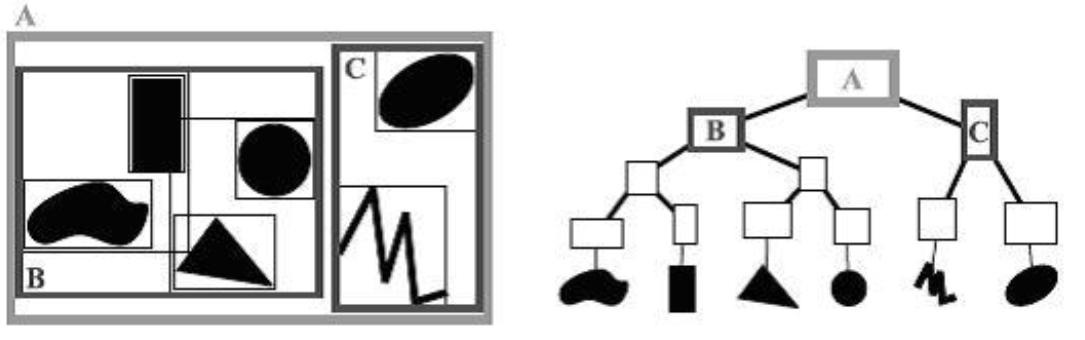
\includegraphics[scale=0.5]{boundingV.jpg}
    \caption[Demonstração de Bounding Volumes Hierárquicos]{Esta figura ilustra o conceito de \textit{Bounding Volumes Hierárquicos}. À esquerda temos uma representação da partição do espaço, e à direita temos a representação sobre a forma de uma árvore. Temos as caixas A, B e C e vários objectos, cada um com a sua caixa.}
\end{figure}

Na nossa implementação de \textit{bounding volumes hierárquicos} permitimos que cada caixa tenha ou não um objecto associado, sendo que no caso de não ter um objecto associado, tem forçosamente de ter caixas-filho que lhe correspondam. Uma caixa que não tenha um objecto associado nem caixas-filho não teria volume, como tal não seria um \textit{Bounding Volume Hierárquico}.

\subsection{Encadeamento de métodos}
O encadeamento de métodos é uma técnica que nos permite criar a árvore de \textit{bounding volumes hierárquicos} (ver secção \ref{bounding volumes hierarquicos}) sem ter de atribuir um elemento a uma variável para o usar.

Para poder utilizar métodos encadeados alterámos os métodos que modificam os elementos de forma a estes nos devolvam o próprio objecto que foi modificado. 

Segue-se um exemplo que ilustra esta técnica.

Suponha-se que temos os seguintes métodos numa classe \textbf{Nodo}:

\begin{verbatim}
Nodo *Nodo::A();
Nodo *Nodo::B(float x, float y, float z);
Nodo *Nodo::C(int valor);
\end{verbatim}

Que modificam um objecto da classe \textbf{Nodo} e devolvem um apontador para um nodo. Inspecionando os métodos, temos que todos eles têm pelo menos um
\begin{verbatim}
return this;
\end{verbatim}
de forma a devolver um apontador para o próprio objecto.

\clearpage
Combinando estas definições com o conceito de árvore, podemos criar uma árvore da forma que abaixo se descreve:

\begin{verbatim}
Nodo *raiz = new Nodo();

raiz
    ->addFilho(
        (new Nodo())->B(1,2,3)->C(9)
            ->addFilho(
                (new Nodo())->A()
            )
     )
    ->addFilho(
        (new Nodo())->C(60)
    );
\end{verbatim}

\clearpage
Desta forma, conseguimos criar a árvore apenas atribuindo valor à variável que representa a raiz da árvore. A árvore gerada teria a seguinte forma:

\begin{verbatim}
Nodo raiz
  |
  |-- Nodo ao qual foi aplicado B(1,2,3) e C(9)
  |     |
  |     `-- Nodo ao qual foi aplicado A()
  |
  `-- Nodo ao qual foi aplicado C(60)
\end{verbatim}

No projecto, a classe \textbf{Nodo} do exemplo corresponde, em parte, à classe \textbf{ObjectTree}.

\newpage
\onecolumn
\section{Organização e Descrição do Projecto}
Pretendemos com esta secção dar a conhecer algumas características mais técnicas sobre o funcionamento da nossa aplicação.

\subsection{Descrição Resumida}
Esta secção visa esclarecer, de uma forma resumida, quanto à funcionalidade de cada classe presente no projecto, assim como as relações entre elas. 
\begin{figure}[!htb]
    \centering
    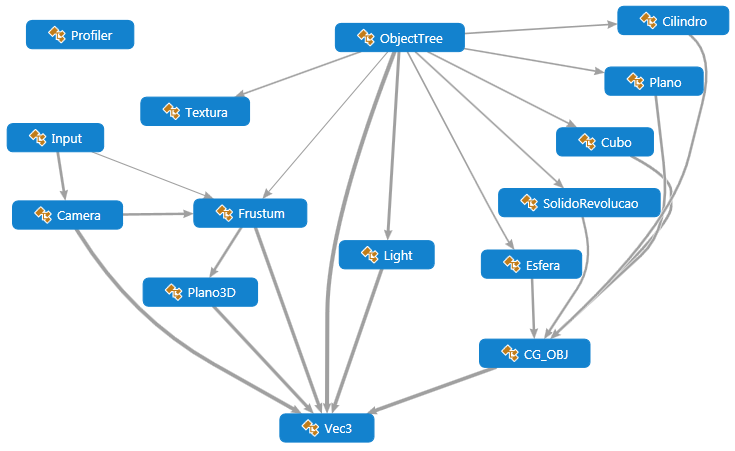
\includegraphics[scale=0.6]{dependencias.png}
    \caption{Relações de inclusão entre as várias classes}
\end{figure}

\clearpage
A classe \textbf{CG\_OBJ} (\ref{classe cg obj}) é onde são definidos os \textit{VBO}s e, portanto, as classes \textbf{Plano} (\ref{classe plano}), \textbf{Cubo} (\ref{classe cubo}), \textbf{Cilindro} (\ref{classe cilindro}), \textbf{Esfera} (\ref{classe esfera}) e \textbf{SolidoRevolucao} (\ref{classe solidorevolucao}) são todas sub-classes desta. O \textbf{Input} (\ref{classe input}) e a \textbf{Camera} (\ref{classe camera}) estão relacionados, pois o movimento do rato modifica os ângulos da orientação da câmara. O \textbf{Input} também controla a activação e desactivação da funcionalidade de \textit{View Frustum Culling} e como tal está relacionada com a classe \textbf{Frustum} (\ref{classe frustum}). A \textbf{Camera} controla quando é que o \textbf{Frustum} deve ser actualizado e efectua essa actualização. A classe \textbf{Frustum} utiliza \textbf{Planos3D} (\ref{classe plano3d}) para definir os limites do \textit{View Frustum}. A iluminação é definida na classe \textbf{Light} (\ref{classe light}) e as texturas na classe \textbf{Textura} (\ref{clsse textura}), ambas são utilizadas pela classe \textbf{ObjectTree} (\ref{classe objecttree}) visto que esta é a classe que agrupa todo o tipo de elementos para construir a cena final. Temos também a classe \textbf{Vec3} (\ref{classe vec3}) que, sendo a definição de um vector com três posições e tratando-se esta de uma aplicação de computação gráfica a três dimensões, é natural que seja utilizada pela maioria das outras classes. Por fim temos a classe \textbf{Profiler} (\ref{clsse profiler}), que não depende de outras componentes do projecto e é apenas utilizada no ficheiro \textbf{main.c}. O ficheiro \textbf{main.c} (\ref{main.c}) e o módulo \textbf{Utilities} (\ref{modulo utilities}) não estão representados no gráfico por não serem classes.

\clearpage
\subsection{Descrição Detalhada}
Esta secção e suas sub-secções explicitam com algum pormenor o funcionamento e propósito dos métodos, propriedades, enumerações e definições das várias classes do projecto.

\subsubsection{Classe Vec3} \label{classe vec3}
Esta classe representa um conjunto de 3 vectores. Tem métodos que permitem que alguns cálculos sejam implementados de uma forma mais legível.

\hfill \\ \underline{\textbf{Propriedades private:}}

\begin{description}
	\item[float vec{[3]}] \hfill \\
	O vector é guardado num array de três elementos.
\end{description}

\hfill \\ \underline{\textbf{Métodos public:}}

\begin{description}
	\item[Vec3()]
	\item[Vec3(Vec3 *elem)]
	\item[Vec3(float A, float B, float C)]
	\item[Vec3(float *vec)] \hfill \\
	Métodos construtores da classe.
	
	\item[Vec3 clone()] \hfill \\
	Método de clone da classe.
	
	\item[float getVal(int pos)] \hfill \\
	Obtém o valor da \textit{pos}-ésima posição do array \textit{vec}.
	
	\item[float X()] \hfill \\
	Obtém o valor da primeira posição do array \textit{vec}.

	\item[float Y()] \hfill \\
	Obtém o valor da segunda posição do array \textit{vec}.
	
	\item[float Z()] \hfill \\
	Obtém o valor da terceira posição do array \textit{vec}.
	
	\item[void setVal(int pos, float val)] \hfill \\
	Coloca o valor \textit{val} na posição \textit{pos} do array \textit{vec}.
	
	\item[void setX(float val)] \hfill \\
	Coloca o valor \textit{val} na primeira posição do array \textit{vec}.
	
	\item[void setY(float val)] \hfill \\
	Coloca o valor \textit{val} na segunda posição do array \textit{vec}.
	
	\item[void setZ(float val)] \hfill \\
	Coloca o valor \textit{val} na terceira posição do array \textit{vec}.
	
	\item[float *getAll(float *arr)] \hfill \\
	Coloca em \textit{arr} os valores do array \textit{vec}.
	
	\item[void reset(float A, float B, float C)] \hfill \\
	Redefine todos os elementos do array \textit{vec}
	
	\item[void incrementar( Vec3 *inc )] \hfill \\
	Soma os valores do objecto actual com os valores do objecto \textit{inc} e substitui os valores do objecto actual pelo resultado da soma.
	
	\item[void decrementar( Vec3 *dec )] \hfill \\
	Subtrai os valores do objecto actual pelos valores do objecto \textit{dec} e substitui os valores do objecto actual pelo resultado da subtracção.
	
	\item[Vec3 somar( Vec3 *vec )] \hfill \\
	Soma os valores do objecto actual com os valores do objecto \textit{vec} e devolve um novo objecto com a soma.
	
	\item[Vec3 multiplicar( float val )] \hfill \\
	Multiplica os valores do objecto actual por um escalar \textit{val} e devolve um novo objecto com o resultado.
	
	\item[Vec3 crossProduct( Vec3 *snd )] \hfill \\
	Calcula o produto externo entre o objecto actual e o objecto \textit{snd}.
	
	\item[float innerProduct( Vec3 *snd)] \hfill \\
	Calcula o produto interno entre o objecto actual e o objecto \textit{snd}.
	
	\item[void normalizar()] \hfill \\
	Normaliza o array \textit{vec}. Ou seja, divide cada uma das posições por ($\sqrt{x^{2}+y^{2}+z^{2}}$)
	
	\item[float norma()] \hfill \\
	Devolve a norma do objecto actual ($\sqrt{x^{2}+y^{2}+z^{2}}$).
\end{description}

\clearpage
\subsubsection{Classe Light} \label{classe light}
Esta classe controla a iluminação no \textit{openGL}. Parte da classe (os métodos static) são apenas alternativas às funções do \textit{openGL} para definir propriedades das luzes do \textit{openGL}. Os outros métodos e as propriedades permitem agrupar um conjunto de definições relativas à iluminação de modo a permitir a	static bool keyDown[256];

\hfill \\ \underline{\textbf{Propriedades private:}}

\begin{description}
	\item[Vec3 pos] \hfill \\
	Localização da luz.

	\item[float D] \hfill \\
	Localização da luz (quarta componente das coordenadas homogéneas).

	\item[Vec3 amb] \hfill \\
	Cor da componente ambiente da luz.

	\item[Vec3 dif] \hfill \\
	Cor da componente difusa da luz.

	\item[Vec3 esp] \hfill \\
	Cor da componente especular da luz.

	\item[Vec3 dir] \hfill \\
	Direcção da luz, caso seja um foco de luz.

	\item[float sExp] \hfill \\
	Intendidade da luz (0-128).

	\item[float sCutOff] \hfill \\
	Abertura da luz ([0-90] ou o valor especial 180)

	\item[GLenum nr] \hfill \\
	Número da luz do \textit{openGL} a que corresponde a luz actual
\end{description}

\hfill \\ \underline{\textbf{Métodos public:}}

\begin{description}
	\item[static void posicao(GLenum light, float x, float y, float z, float w)] \hfill \\
	Define a posição de uma determinada luz do \textit{openGL}.

	\item[static void ambiente(GLenum light, float r, float g, float b)] \hfill \\
	Define a componente ambiente de uma determinada luz do \textit{openGL}.

	\item[static void difusa(GLenum light, float r, float g, float b)] \hfill \\
	Define a componente difusa de uma determinada luz do \textit{openGL}.

	\item[static void especular(GLenum light, float r, float g, float b)] \hfill \\
	Define a componente especular de uma determinada luz do \textit{openGL}.

	\item[static void direccao(GLenum light, float x, float y, float z)] \hfill \\
	Define a direcção de uma determinada luz direccional do \textit{openGL}.

	\item[static void spotExp(GLenum light, float exp)] \hfill \\
	Intendidade de uma determinada luz do \textit{OpenGL} (0-128).

	\item[static void spotCutOff(GLenum light, float cutOff)] \hfill \\
	Abertura de uma determinada luz do \textit{openGL} ([0-90] ou o valor especial 180).

	\item[static void enable(GLenum light)] \hfill \\
	Liga uma determinada luz do \textit{openGL}.

	\item[static void disable(GLenum light)] \hfill \\
	Desliga uma determinada luz do \textit{openGL}.

	\item[Light()]
	\item[Light(LuzId id)] \hfill \\
	Construtores da classe.
	
	\item[Light *setPos(Vec3 pos, float D)] \hfill \\
	Define a posição do objecto \textbf{Light}.

	\item[Light *setAmb(Vec3 amb)] \hfill \\
	Define a componente ambiente do objecto \textbf{Light}.

	\item[Light *setDif(Vec3 dif)] \hfill \\
	Define a componente difusa do objecto \textbf{Light}.

	\item[Light *setEsp(Vec3 esp)] \hfill \\
	Define a componente especular do objecto \textbf{Light}.

	\item[Light *setDir(Vec3 dir)] \hfill \\
	Define a direcção do objecto \textbf{Light}.

	\item[Light *setSpotExp(float exp)] \hfill \\
	Define a intensidade do objecto \textbf{Light}.

	\item[Light *setSpotCutOff(float cutOff)] \hfill \\
	Define a abertura do objecto \textbf{Light}.

	\item[void aplicarELigar()] \hfill \\
	Aplica as propriedades definidas para o actual objecto \textbf{Light} à luz do \textit{openGL} que lhe está associada e liga essa luz.

	\item[void desligar()] \hfill \\
	Desliga a luz do openGL associada ao objecto \textbf{Light}.
\end{description}

\clearpage
\subsubsection{Classe Input} \label{classe input}
A classe \textbf{Input} é a classe essencial para a gestão de input.

\hfill \\ \underline{\textbf{Propriedades private:}}

\begin{description}
	\item[static bool keyDown{[256]}] \hfill \\
	Array de 256 posições que tem o valor \textit{true} se a posição associdada a uma determinada tecla estiver pressionada.
\end{description}

\hfill \\ \underline{\textbf{Métodos e propriedades public:}}

\begin{description}
	\item[static void init()] \hfill \\
	Definir funções para \textit{glutKeyboardFunc}, \textit{glutKeyboardUpFunc}, entre outras.

	\item[static void keyPress(unsigned char tecla, int x, int y)] \hfill \\
	Realiza acções para algumas teclas e define o \textit{keyDown} no índice correspondente à tecla pressionada a \textit{true}.

	\item[static void KeyUp(unsigned char tecla, int x, int y)] \hfill \\
	Coloca o \textit{keyDown} no índice correspondente à tecla solta a \textit{false}.

	\item[static void processInput()] \hfill \\
	Método que executa acções conforme as teclas pressionadas de acordo com o array \textit{keyDown}.

	\item[static bool apenasLinhas] \hfill \\
	Permite alternar entre desenhar os objectos de forma opaca ou apenas os seus limites.
\end{description}

\clearpage
\subsubsection{Classe Camera} \label{classe camera}
Esta classe controla a funcionalidade da câmara FPS no nosso projecto (ver secção \ref{camara fps}).

\hfill \\ \underline{\textbf{Propriedades private:}}

\begin{description}
	\item[static bool modoFPS] \hfill \\
	Permite activar ou desactivar o modo FPS da câmara.

	\item[static Vec3 fpsMousePos] \hfill \\
	Ultima posição do rato antes de desactivar o modo FPS.

	\item[static Vec3 pos] \hfill \\
	Posição da câmara.

	\item[static float alpha]
	\item[static float beta] \hfill \\
	Orientação da câmara.

	\item[static float passo] \hfill \\
	Distância percorrida de cada vez que a câmara se desloca numa determinada direcção.

	\item[static float dnear] \hfill \\
	Distância da câmara ao plano near.

	\item[static float dfar] \hfill \\
	Distância da câmara ao plano far.

	\item[static float fov] \hfill \\
	Parâmetro fov da função gluPerspective.

	\item[static float ratio] \hfill \\
	Rácio entre o comprimento e a largura da janela.

	\item[static Vec3 up] \hfill \\
	Vector up, como definido na função gluLookAt.

	\item[static Vec3 center] \hfill \\
	Ponto para onde a câmara está apontada
\end{description}

\hfill \\ \underline{\textbf{Métodos public:}}

\begin{description}
	\item[static void init(float x, float y, float z)] \hfill \\
	Inicializa a câmara numa determinada posição.

	\item[static void lookAt()] \hfill \\
	Método que utiliza a função gluLookAt de acordo com as propriedades da câmara.

	\item[static void toggleFPS()] \hfill \\
	Alterna entre o modo FPS e o modo sem controlo sobre a orientação da câmara.

	\item[static void changeSize(int w, int h)] \hfill \\
	Método que é chamado quando a janela é redimensionada.

	\item[static void moverFrente()]
	\item[static void moverTras()]
	\item[static void moverEsquerda()]
	\item[static void moverDireita()]
	\item[static void moveTo(float x, float y, float z)] \hfill \\
	Movimento da câmara nas várias direcções ou para um ponto específico.

	\item[static void mouseMove(int x, int y)] \hfill \\
	Actualizar os ângulos da orientação da câmara de acordo com a posição actual do rato.

	\item[static void lookAt(float x, float y, float z)] \hfill \\
	Forçar a câmara a apontar para um determinado ponto.

	\item[static void passoMaior()] \hfill \\
	Aumentar a velocidade de movimento da câmara.

	\item[static void passoMenor()] \hfill \\
	Reduzir a velocidade de movimento da câmara.

	\item[static void setOrthographicProjection()] \hfill \\
	Muda para a matriz de Projecção para escrever texto.

	\item[static void restorePerspectiveProjection()] \hfill \\
	Muda para a matriz Model View Projection.

	\item[static void renderString( float x, float y, int spacing, Fonts font, char *string)] \hfill \\
	Escreve um texto no ecrã na posição $(x,y)$ com um determinado espaçamento extra ente caracteres e o tipo de letra especificado.
\end{description}

\clearpage
\subsubsection{Classe CG\_OBJ} \label{classe cg obj}
Método que permite implementar \textit{VBO}s (ver secção \ref{VBO}).

Todas as primitivas e sólidos de revolução são sub-classes desta classe. Desta forma o comportamento de um \textit{VBO} é homogéneo e obtemos maior escalabilidade.

\hfill \\ \underline{\textbf{Métodos e propriedades private:}}

\begin{description}
	\item[static int maxBuffers]
	\item[static int nBuffers] \hfill \\
	Número máximo de buffers e o número de buffers em utilização.

	\item[void addVertex(int *indice, float x, float y, float z)]
	\item[void addNormal(int *indice, float x, float y, float z)]
	\item[void addTextureCoord(int *indice, float x, float y)]
	\item[void addVertex(int *indice, float x1, float y1, float z1, float x2, float y2,]
	\item[float z2, float x3, float y3, float z3)]
	\item[void addNormal(int *indice, float x1, float y1, float z1, float x2, float y2,]
	\item[float x3, float y3, float z3)]
	\item[void addTextureCoord(int *indice, float x1, float y1, float x2, float y2,]
	\item[float x3, float y3)] \hfill \\
	Adiciona vértices, normais ou coordenadas de textura aos arrays de vértices, normais ou coordenadas de textura, respectivamente.

	\item[float comprimento] \hfill \\
	Comprimento dos sólidos de revolução.

	\item[void calculateBounds()] \hfill \\
	Calcula os limites da caixa que deve envolver o objecto.

	\item[int nTriangulos]
	\item[int nVertices]
	\item[int nFloats] \hfill \\
	Número de triângulos, vértices e valores de vírgula flutuante do objecto.

	\item[int bufferPos   // posição no buffer onde está o objecto] \hfill \\
	Número do primeiro \textit{Vertex Object Buffer} onde está guardado o objecto.

	\item[float *vertexB  // array de coordenadas]
	\item[float *normalB  // array de normais]
	\item[float *textureB // array de coordenadas de textura] \hfill \\
	Arrays de coordenadas, normais e coordenadas de textura, respectivamente.

	\item[int *vertexI    // array de indices de coordenadas] \hfill \\
	Array de índices de coordenadas.

	\item[void guardarOBJ(int nTriangulos)] \hfill \\
	Método que inicializa alguns valores para depois ser preenchido o array de coordenadas, normais e coordenadas de textura.

	\item[virtual void preencherVertices()] \hfill \\
	Método que preenche os arrays de vértices, normais e coordenadas de textura. Este método é implementado por todas as subclasses da classe \textbf{CG\_OBJ}, isto porque cada objecto é composto por diferentes vértices.

	\item[void revolutionSolidClose(float *x, float *y, int count, int fatias)]
	\item[void revolutionSolidOpen(float *x, float *y, int count, int fatias)] \hfill \\
	Preenche o array de vértices de acordo com as coordenadas XY e constroi um sólido de revolução. 

	\item[Vec3 emissiva]
	\item[Vec3 especular]
	\item[Vec3 ambiente]
	\item[Vec3 difusa]
	\item[float shininess] \hfill \\
	Propriedades do material.
\end{description}

\hfill \\ \underline{\textbf{Métodos e propriedades public:}}

\begin{description}
	\item[static GLuint *buffers] \hfill \\
	Array de indentificadores de Vertex Buffer Objects.

	\item[static void prepararBuffer(int maxBuffers)] \hfill \\
	Aloca espaço e preenche o array de identificadores de VBOs.

	\item[void preencherIndices()] \hfill \\
	Identifica os vértices que ocorrem mais que uma vez no objecto e preenche o array de Indices de acordo com essa informação.

	\item[void desenhar()] \hfill \\
	Desenha o objecto.

	\item[static int getMaxBuffers()] \hfill \\
	Obtém o número máximo de buffers disponíveis.

	\item[Vec3 *minBound]
	\item[Vec3 *maxBound] \hfill \\
	Obtém os limites do objecto nos vários eixos.

	\item[CG\_OBJ *setEmissiva(float r, float g, float b)]
	\item[CG\_OBJ *setEspecular(float r, float g, float b)]
	\item[CG\_OBJ *setAmbiente(float r, float g, float b)]
	\item[CG\_OBJ *setDifusa(float r, float g, float b)]
	\item[CG\_OBJ *setShininess(float s)] \hfill \\
	Permite defenir as propriedades do material com a possibilidade de encadeamento de métodos.
\end{description}

\clearpage
\subsubsection{Classe Plano} \label{classe plano}
Classe que implementa a construção de um plano. Sub-classe da classe CG\_OBJ (ver secção \ref{classe cg obj}).

\hfill \\ \underline{\textbf{Métodos e propriedades private:}}

\begin{description}
	\item[int camadasx] \hfill \\
	Número de camadas no eixo dos $xx$.

	\item[int camadasz] \hfill \\
	Número de camadas no eixo dos $zz$.

	\item[float comprimento] \hfill \\
	Comprimento no eixo dos $xx$.

	\item[float largura] \hfill \\
	Comprimento no eixo dos $zz$.

	\item[void preencherVertices()] \hfill \\
	Implementação específica para o plano do método preencherVertices.
\end{description}

\hfill \\ \underline{\textbf{Métodos public:}}

\begin{description}
	\item[Plano(float comprimento, int camadasx, int camadasz)]
	\item[Plano(float compX, float compZ, int camadasx, int camadasz)] \hfill \\
	Construtores da classe.
\end{description}

\clearpage
\subsubsection{Classe Cubo} \label{classe cubo}
Classe que implementa a construção de um paralelipípedo. Sub-classe da classe CG\_OBJ (ver secção \ref{classe cg obj}).

A classe chama-se \textbf{Cubo} porque começou por construir cubo ao qual aplicávamos escalas em determinados eixos para o transformar num paralelipípedo. Na ultima fase decidimos que seria mais fácil arranjar uma forma de construir um paralelipípedo e não achámos que existisse uma grande necessidade de substituir o nome original da classe.

Apesar destas modificações, a classe \textbf{Cubo} continua a ter um construtor que recebe o lado em vez dos vários comprimentos, construindo assim um cubo.

\hfill \\ \underline{\textbf{Métodos e propriedades private:}}

\begin{description}
	\item[int camadasx]
	\item[int camadasy]
	\item[int camadasz] \hfill \\
	Número de camadas nos vários eixo

	\item[float compX]
	\item[float compY]
	\item[float compZ] \hfill \\
	Comprimento do cubo nos vários eixos. Apenas se todos os comprimentos forem iguais é que é realmente um cubo.

	\item[void preencherVertices()] \hfill \\
	Implementação específica para o cubo do método preencherVertices.
\end{description}

\hfill \\ \underline{\textbf{Métodos public:}}

\begin{description}
	\item[Cubo(float lado, int camadasx, int camadasy, int camadasz);]
	\item[Cubo(float compX, float compY, float compZ, int camadasx, int camadasy, int camadasz)] \hfill \\
	Construtores da classe.
\end{description}

\clearpage
\subsubsection{Classe Cilindro} \label{classe cilindro}
Classe que implementa a construção de um cilindro. Sub-classe da classe CG\_OBJ (ver secção \ref{classe cg obj}).

\hfill \\ \underline{\textbf{Métodos e propriedades private:}}

\begin{description}
	\item[float raio] \hfill \\
	Raio do cilindro.

	\item[float altura] \hfill \\
	Altura do cilindro.

	\item[int fatias] \hfill \\
	Número de fatias do cilindro.

	\item[int seccoes] \hfill \\
	Número de secções verticais do cilindro

	\item[void preencherVertices()] \hfill \\
	Implementação específica para o cubo do método preencherVertices.
\end{description}

\hfill \\ \underline{\textbf{Métodos public:}}

\begin{description}
	\item[Cilindro(float raio, float altura, int fatias, int seccoes)] \hfill \\
	Construtor da classe.
\end{description}

\clearpage
\subsubsection{Classe Esfera} \label{classe esfera}
Classe que implementa a construção de uma esfera. Sub-classe da classe CG\_OBJ (ver secção \ref{classe cg obj}).

\hfill \\ \underline{\textbf{Métodos e propriedades private:}}

\begin{description}
	\item[float raio] \hfill \\
	Raio da esfera.

	\item[int fatias] \hfill \\
	Número de fatias da esfera.

	\item[int seccoes] \hfill \\
	Número de secções da esfera.

	\item[void preencherVertices()] \hfill \\
	Implementação específica para o cubo do método preencherVertices.
\end{description}

\hfill \\ \underline{\textbf{Métodos public:}}

\begin{description}
	\item[Esfera(float raio, unsigned fatias, unsigned seccoes)] \hfill \\
	Construtor da classe.
\end{description}

\clearpage
\subsubsection{Classe SolidoRevolucao} \label{classe solidorevolucao}
Classe que implementa a construção de um sólido de revolução. Sub-classe da classe CG\_OBJ (ver secção \ref{classe cg obj}).

\hfill \\ \underline{\textbf{Enumerações:}}

\begin{description}
	\item[enum TipoSolidoRevolucao] \hfill \\
	Forma de identificar os vários tipos de sólidos de revolução que podem ser criados com esta classe.
\end{description}

\hfill \\ \underline{\textbf{Métodos e propriedades private:}}

\begin{description}
	\item[int fatias] \hfill \\
	Número de fatias.

	\item[bool fechado] \hfill \\
	Propriedade que indica se o sólido de revolução deve ser fechado ou se tem uma abertura no meio.

	\item[float x{[100]}]
	\item[float y{[100]}]\hfill \\
	Arrays que permitem guardar 100 pontos na forma $(x,y)$

	\item[int pontos] \hfill \\
	Número de pontos sobre a forma $(x,y)$ com valores definidos.

	\item[void preencherVertices()] \hfill \\
	Implementação específica para os sólidos de revolução do método preencherVertices.
\end{description}

\hfill \\ \underline{\textbf{Métodos public:}}

\begin{description}
	\item[SolidoRevolucao(TipoSolidoRevolucao tipo, int detalhe)] \hfill \\
	Construtor da classe.
\end{description}

\clearpage
\subsubsection{Classe Plano3D} \label{classe plano3d}
A classe \textbf{Plano3D} permite guardar informação sobre um plano definido a 3 dimensões.

\hfill \\ \underline{\textbf{Propriedades private:}}

\begin{description}
	\item[Vec3 normal] \hfill \\
	Normal do plano.

	\item[float D] \hfill \\
	Distância do plano à origem.

	\item[Vec3 ponto] \hfill \\
	Ponto no plano.
\end{description}

\hfill \\ \underline{\textbf{Métodos public:}}

\begin{description}
	\item[Plano3D()]
	\item[Plano3D( Vec3 *normal, Vec3 *ponto )] \hfill \\
	Construtores da classe.

	\item[Vec3 getPonto()] \hfill \\
	Obter o ponto no plano.

	\item[Vec3 getNormal()] \hfill \\
	Obter a normal do plano.

	\item[float distancia( Vec3 *ponto )] \hfill \\
	Obter a distância do plano à origem.
\end{description}

\clearpage
\subsubsection{Classe Frustum} \label{classe frustum}
Classe que define os planos do \textit{View Frustum} e que permite indetificar as caixas que estão dentro, fora ou a intersectar o \textit{View Frustum}.

\hfill \\ \underline{\textbf{Enumerações:}}

\begin{description}
	\item[enum PlanosFrustum] \hfill \\
	Forma de identificar os vários planos do \textit{frustum}.
	\item[enum PosicaoNoFrustum] \hfill \\
	Forma de identificar a posição de uma caixa em relação ao \textit{frustum}.
\end{description}

\hfill \\ \underline{\textbf{Métodos e propriedades private:}}

\begin{description}
	\item[static bool frustumNeedsUpdate] \hfill \\
	Permite saber se o frustum precisa de ser actualizado (devido ao movimento da câmara).

	\item[static bool frustumCullingEnabled] \hfill \\
	Permite saber se o \textit{View Frustum Culling} está activado.

	\item[static Plano3D plano{[planoCOUNT\_ENUM]}] \hfill \\
	Os vários planos do \textit{frustum}.

	\item[static bool pointInFrustum(Vec3 *ponto)] \hfill \\
	Verifica se um ponto se encontra dentro do \textit{view frustum}.
\end{description}

\hfill \\ \underline{\textbf{Métodos public:}}

\begin{description}
	\item[static void updateFrustum( Vec3 *pos, Vec3 *up, Vec3 *center, float fov]
	\item[float ratio, float dNear, float dFar)] \hfill \\
	Actualiza os planos do frustum de acordo com os parâmetros da câmara.

	\item[static PosicaoNoFrustum boxInFrustum(Vec3 *min, Vec3 *max)] \hfill \\
	Verifica se uma caixa está dentro, fora ou a intersectar o view frustum.

	\item[static void toggleFrustumCulling()] \hfill \\
	Activar e desactivar o \textit{View Frustum Culling}.

	\item[static bool isCullingEnabled()] \hfill \\
	Verifica se o \textit{View Frustum Culling} está activo.

	\item[static void scheduleUpdate()] \hfill \\
	Informa a classe que os planos do frustum precisam de ser atualizados.
\end{description}

\clearpage
\subsubsection{Classe ObjectTree} \label{classe objecttree}
Esta classe organiza os elementos visuais do nosso projecto sob a forma de uma árvore (ver secção \ref{bounding volumes hierarquicos} sobre \textit{Bounding Volumes Hierárquicos}). Esta classe também desenha toda a cena percorrendo a árvore da raiz para as folhas.

\hfill \\ \underline{\textbf{Enumeração:}}

\begin{description}
	\item[enum TipoMod] \hfill \\
	Forma de identificar os vários tipos de modificações: translações, rotações e escalas.
\end{description}

\hfill \\ \underline{\textbf{Métodos e propriedades private:}}

\begin{description}
	\item[int modsCount] \hfill \\
	Número de modificações efectuadas no objecto.

	\item[TipoMod *modsTipo] \hfill \\
	Array do tipo de modificações.

	\item[Vec3 *modsVec] \hfill \\
	Array de vectores das modificações.

	\item[float *modsExtra] \hfill \\
	Array de ângulos necessários para efectuar rotações.

	\item[bool texturizar] \hfill \\
	Indica se ao objecto deve ser aplicada uma textura.

	\item[Vec3 cor] \hfill \\
	Indica a cor do objecto caso não seja implementada uma textura.

	\item[TipoTextura texTipo] \hfill \\
	Tipo da textura a aplicar ao objecto.

	\item[float texScaleX, texScaleY, texAnguloRotacao] \hfill \\
	Escalas e ângulo de rotação da textura a aplicar.

	\item[Light *luzes[8]] \hfill \\
	Luzes que irão iluminar o objecto.

	\item[CG\_OBJ *obj] \hfill \\
	O objecto a desenhar.

	\item[Vec3 *boundsMin] \hfill \\
	Os limites inferiores do objecto e dos filhos nos vários eixos.

	\item[Vec3 *boundsMax] \hfill \\
	Os limites superiores do objecto e dos filhos nos vários eixos.
	
	\item[bool *toggle] \hfill \\
	Activar ou desactivar o desenho do objecto.

	\item[int numFilhos] \hfill \\
	Número de filhos que o objecto tem.

	\item[ObjectTree **filhos] \hfill \\
	Array de filhos do objecto.

	\item[static ObjectTree *raizObj] \hfill \\
	A raiz da árvore.

	\item[static void drawAux(ObjectTree *raiz, PosicaoNoFrustum posNoFrustum)] \hfill \\
	Desenhar o objecto caso este esteja no \textit{frustum}. Fazer a mesma operação para todos os filhos do objecto. Ver \ref{classe frustum} sobre a classe Frustum.

	\item[static void checkBounds(ObjectTree *tree)] \hfill \\
	Verificar recursivamente os limites dos vários objectos da árvore.

	\item[static void localEfectivo(ObjectTree *tree, Vec3 *ponto)] \hfill \\
	Modifica o ponto de acordo com as rotações, translações e escalas associadas ao objecto.

	\item[static Light *luzesGlobais{[8]}] \hfill \\
	Definição de luzes globais a todos os objectos.
\end{description}

\hfill \\ \underline{\textbf{Métodos e propriedades public:}}

\begin{description}
	\item[ObjectTree()] \hfill \\
	Construtor da classe.

	\item[ObjectTree *rotate( float angulo, Vec3 vec )]
	\item[ObjectTree *translate( Vec3 vec )]
	\item[ObjectTree *scale( Vec3 vec )] \hfill \\
	Adiciona uma modificação ao objecto.

	\item[ObjectTree *color( Vec3 vec )] \hfill \\
	Define a cor do objecto.

	\item[ObjectTree *texture(TipoTextura tipo, float sX, float sY, float anguloRot)] \hfill \\
	Define a textura do objecto.

	\item[ObjectTree *addLight( Light *luz )] \hfill \\
	Adiciona uma luz ao objecto.

	\item[ObjectTree *addLights( Light *luzes{[]}, int i0=-1, int i1=-1, int i2=-1]
	\item[int i3=-1, int i4=-1, int i5=-1, int i6=-1, int i7=-1)] \hfill \\
	Selecciona as luzes a adicionar ao objecto a partir de um array de luzes.

	\item[ObjectTree *objecto( CG\_OBJ *O )] \hfill \\
	Adiciona uma figura ao actual nodo da árvore.

	\item[ObjectTree *addFilho( ObjectTree *filho )] \hfill \\
	Adiciona um filho ao actual nodo da árvore.

	\item[static void init()] \hfill \\
	Inicializa algumas variáveis e prossegue para inicializar toda a toda a árvore recorrendo a encadeamento de métodos. Por fim calcula os limites (i.e as caixas) para cada nodo da árvore.

	\item[static void draw()] \hfill \\
	Desenhar a árvore. Este método apenas inicia o desenho recursivo da árvore começando pela raiz.
\end{description}

\clearpage
\subsubsection{Classe Profiler} \label{clsse profiler}
Esta classe permite a cronometragem de determinadas tarefas. Na quarta fase a classe apenas é utilizada para calcular as frames por segundo da aplicação. Ao longo do desenvolvimento do projecto, esta classe foi utilizada para medir e comparar os tempos de implementações alternativas para nos auxiliar numa tomada de decisão.

\hfill \\ \underline{\textbf{Enumerações:}}

\begin{description}
	\item[enum ProfilerData] \hfill \\
	Forma de identificar os vários cronómetros existentes.
\end{description}

\hfill \\ \underline{\textbf{Propriedades private:}}

\begin{description}
	\item[static int *cronometros] \hfill \\
	Array de tempos, para poder manter registo de vários cronómetros simultaneamente.

	\item[static int *emPausa] \hfill \\
	Array que indica se o cronometro correspondente no array de cronómetros está em pausa e quanto tempo tinha contado antes de ter sido posto em pausa.

	\item[static int frames] \hfill \\
	Valor utilizado para calcular as frames por segundo.

	\item[static float fps] \hfill \\
	Ultimo valor calculado para frames por segundo.
\end{description}

\hfill \\ \underline{\textbf{Métodos public:}}

\begin{description}
	\item[static void init()] \hfill \\
	Alocar espaço para os vários cronómetros.

	\item[static int diff(ProfilerData cronometro)] \hfill \\
	Calcula quanto tempo já passou desde que o cronómetro foi iniciado.

	\item[static void start(ProfilerData cronometro)] \hfill \\
	Iniciar ou continuar um cronómetro.

	\item[static void pause(ProfilerData cronometro)] \hfill \\
	Pausar um cronómetro. Consiste em guardar o tempo actual e adicioná-lo ao cronómetro da próxima vez que este for iniciado.

	\item[static int now()] \hfill \\
	Obtém o tempo sob a forma de número de milisegundos que passaram desde a chamada à função glutInit.

	\item[static void startFrame()] \hfill \\
	Actualiza o contador de frames que passaram no segundo actual e, caso já tenha passado um segundo completo, regista quantas frames foram desenhadas.

	\item[static float getFPS()] \hfill \\
	Obter o número de frames por segundo (valor diz respeito ao ultimo segundo).
\end{description}

\clearpage
\subsubsection{Classe Textura} \label{clsse textura}
A classe \textbf{Textura} permite carregar e utilizar diversas texturas no nosso bar.

\hfill \\ \underline{\textbf{Enumerações:}}

\begin{description}
	\item[enum TipoTextura : int] \hfill \\
	Forma de identificação das várias texturas.
\end{description}

\hfill \\ \underline{\textbf{Propriedades e métodos private:}}

\begin{description}
	\item[static GLuint *textureIds] \hfill \\
	Identificadores de textura.

	\item[static Textura *texturas] \hfill \\
	Objectos do tipo Textura que permitem aplicar a textura a uma figura.

	\item[static ILuint *imageIds] \hfill \\
	Identificadores de imagem.

	\item[static char **filenames] \hfill \\
	Array de string que guarda o nome do ficheiro fonte.

	\item[int tw, th] \hfill \\
	O comprimento e largura da imagem fonte.

	\item[ILubyte *imageData] \hfill \\
	Identificador da imagem importada.

	\item[Textura(TipoTextura tipoTextura)] \hfill \\
	Construtor da classe.
\end{description}

\hfill \\ \underline{\textbf{Métodos public:}}

\begin{description}
	\item[static void init()] \hfill \\
	Carrega as imagens e converte-as para texturas do openGL.

	\item[static int getWidth(TipoTextura tipoTextura)]
	\item[static int getHeight(TipoTextura tipoTextura)] \hfill \\
	Obter o comprimento e largura de uma imagem.

	\item[static void setTextura(TipoTextura tipoTextura, float sx=1, float sy=1, float graus=0)] \hfill \\
	Aplicar uma textura com uma determinada escala e rotação.

	\item[static void setTextura(float sx, float sy, float graus=0)] \hfill \\
	Aplica uma escala e rotação à textura previamente seleccionada.

	\item[static void setColor(float R, float G, float B)] \hfill \\
	Aplicar uma cor RGB em vez de uma textura.

	\item[static void translate(float x, float y)] \hfill \\
	Aplica uma translação à textura.

	\item[static void unsetTextura()] \hfill \\
	Activar a textura "vazia" do openGL.

	\item[int getWidth()]
	\item[int getHeight()] \hfill \\
	Obter o comprimento e a largura da textura.
\end{description}

\clearpage
\subsubsection{Módulo Utilities} \label{modulo utilities}
Nas fases anteriores, este módulo tinha várias funções relacionadas com cálculo algébrico, mas com a introdução da classe \textbf{Vec3} na fase final do projecto, esses cálculos passaram a ser feitos na nova classe. O que restou nesta classe foram duas definições.

\hfill \\ \underline{\textbf{Definições:}}

\begin{description}
	\item[toDegree(rad)]
	\item[toRadian(deg)] \hfill \\
	Converter radianos em graus e o processo inverso. Os números apresentados na definição correspondem a uma aproximação de $\frac{180}{\pi}$ e $\frac{\pi}{180}$, respectivamente.
\end{description}

\clearpage
\subsubsection{Ficheiro main.c} \label{main.c}


\hfill \\ \underline{\textbf{Funções:}}

\begin{description}
	\item[renderScene] \hfill \\
	A função renderScene pede à classe \textbf{Input} para interpretar qualquer input, indica à classe \textbf{Profiler} que está a ser desenhada uma nova frame e prossegue para o desenho da cena, que é feito através de uma chamada ao método draw da classe \textbf{ObjectTree}. Depois do desenho da cena é escrito o valor correspondente às frames por segundo no canto superior direito do ecrã e são trocados os buffers de desenho.
	
	\item[main] \hfill \\
	A função main inicializa todo o tipo de variáveis que podem ser inicializadas em modo \textit{offline} e entrega o controlo da aplicação ao glut.
\end{description}


\clearpage
\section{Conclusão}
Fazendo uma retrospectiva ao projecto por nós desenvolvido, pensamos ter cumprido os requisitos exigidos para a aplicação, assim como algumas funcionalidades que implementámos para melhorar o nosso produto final.

Todos os pontos exigidos no enunciado foram cumpridos para as correspondentes fases com alguma facilidade, à excepção da fase final. Este facto deve-se, por um lado, à nossa implementação parcial de \textit{VBO}s na segunda fase e assim reduzir a quantidade de funcionalidades a implementar na terceira fase. Por outro lado o tempo foi escasso para realizar a quarta fase, com a agravante de termos começado a implementar um modo de desenho do bar que, além de não ser facilmente escalável, acabou por se provar ineficiente. Este contratempo deixou-nos com apenas uma semana para compor o bar utilizando uma outra qualquer implementação. De forma a valorizar o projecto, decidimos implementar \textit{View Frustum Culling} com \textit{Bounding Volumes Hierárquicos}. Talvez esta ultima decisão tenha contribuido para o atraso na entrega do nosso bar, mas consideramos que o que mais nos prejudicou em termos de tempo foi a nossa primeira tentativa (falhada) de desenhar o bar. Esta decisão de utilizar \textit{View Frustum Culling} com \textit{Bounding Volumes Hierárquicos} também foi um desafio que, depois de superado, nos proporcionou uma aprendizagem mais completa na área da computação gráfica.

Desde o início do projecto houve uma grande preocupação da nossa parte em ter o projecto bem organizado, orientado a objectos e extremamente escalável. Esta preocupação deve-se a alguma experiência prévia em programação orientada a objectos e a consciência de que seria sempre muito mais fácil acrescentar novas funcionalidades a um projecto escalável e orientado a objectos. Um exemplo desta nossa preocupação é a classe \textbf{CG\_OBJ}, que controla todos os aspectos referentes aos \textit{VBO}s à excepção da introdução de vértices. Esta parte crucial da definição de um \textit{VBO}, a introdução dos vértices, é feita de uma forma dinâmica através da definição de um método abstracto (ou virtual, em C++) em todas as sub-classes de \textbf{CG\_OBJ}. Outro exemplo é a forma como são definidas as texturas, que nos permitem adicionar uma nova textura especificando apenas um nome para a textura e a sua localização em disco. Foi também tido algum cuidado para manter um equilíbrio no que diz respeito a optimizações numa fase de desenvolvimento do projecto. Tentámos não optimizar o código, mas ao mesmo tempo não utilizar técnicas pouco eficientes.

Podemos então afirmar que o desenvolvimento desde projecto foi concluído, no entanto reconhecemos que poderiam ter sido aplicadas mais optimizações e técnicas no projecto, como por exemplo a redução do numero de mudanças de estado antes do desenho de cada objecto, uma melhor divisão dos objectos pela Hierarquia de Volumes ou a introdução de sombras.


\clearpage
\section{Referências}

\subsection{Referências bibliográficas}
\begin{description}
	\item[Slides teóricos e práticos] \hfill \\
	Slides mostrados durante as aulas de Computação Gráfica.
\end{description}

\subsection{Referências WWW}
\begin{description}
	\item[www.lighthouse3d.com] \hfill \\
	Lighthouse3D is a site devoted mostly to 3D computer graphics.
\end{description}

\clearpage
\onecolumn
\section{Membros do Grupo}
\begin{center}
    \begin{tabular}{ccc}
        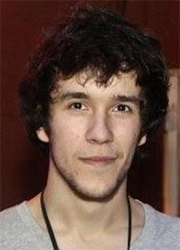
\includegraphics[scale=0.5]{bruno.png}&
        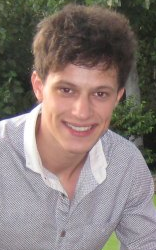
\includegraphics[scale=0.5]{serafim.png}\\
        
        \small{\textbf{Bruno Ferreira}}&
        \small{\textbf{Serafim Pinto}}\\
        \small{\textbf{A61055}}&
        \small{\textbf{A61056}}\\
    \end{tabular}
\end{center}
\end{document}